\section{Efficient Equality Saturation for the Lambda Calculus} %\todo{nice is this section starts on page 12}
\label{eqsat-bindings}


\begin{table}
  \begin{tabular}{|c|c|c|}
  \hline
  \textbf{$\bm{\lambda}$ calculus} & $\bm{F}$ & $\bm{t_1, .., t_n}$ \\
  \hline
  \begin{rise}[numbers=none, frame=none]
  $\lambda$x. e
  \end{rise}%
  & lam x & e \\
  \hline
  \begin{rise}[numbers=none, frame=none]
  e$_1$ e$_2$
  \end{rise}%
  & app & e$_1$, e$_2$ \\
  \hline
  \begin{rise}[numbers=none, frame=none]
  x
  \end{rise}%
  & var x & \\
  \hline
  \end{tabular}
  \caption{Encoding of $\lambda$ calculus terms as $F(t_1, .., t_n)$ terms for the purposes of equality saturation.}
  \label{fig:rise-node-repr}
  \end{table}

\begin{figure}
\begin{align*}
    \tag{$\beta$-reduction}\label{beta-reduction}
    ({\color{cyan}\lambda x.}~b)~e \rewritesTo{}& {\color{purple}b[e/x]} \\
    \tag{$\eta$-reduction}\label{eta-reduction}
    {\color{cyan}\lambda x.}~f~x \rewritesTo{}& f &{\color{orange}\text{if}~x~\text{not free in}~f} \\
    \tag{map-fusion}\label{map-fusion}
    map~f~{\color{gray}(}map~g~{\color{gray}arg)} \rewritesTo{}& map~{\color{gray}({\color{cyan}\lambda x.}}~f~{\color{gray}(}g~{\color{gray}x))~arg} \\
    \tag{map-fission}\label{map-fission}
    map~{\color{gray}({\color{cyan}\lambda x.}}~f~gx) \rewritesTo{}& {\color{gray}{\color{cyan}\lambda y.}}~map~f~{\color{gray}(}map~{\color{gray}({\color{cyan}\lambda x.}}~gx{\color{gray})~y)}
    &{\color{orange}\text{if}~x~\text{not free in}~f}
\end{align*}%}
\caption{\Rise{} rewrite rules using {\color{purple}substitution}, {\color{cyan}name bindings} (lambda abstractions), and {\color{orange} freshness predicates}.}
\label{fig:example-rules}
\end{figure}

We now investigate the second direction shown in \cref{fig:overview} for scaling equality saturation to complex optimizations of functional programs, by exploring the engineering design choices required to efficiently encode a polymorphically typed lambda calculus within equality saturation.
A set of design choices are realized for the \Rise{} language in the new \kles{} implementation that is heavily inspired by the egg library \cite{willsey2021-egg}.

Lambda calculus terms can be encoded as terms of shape $F(t_1, .., t_n)$, as shown in \cref{fig:rise-node-repr}.
Variable names are not modeled directly as terms, but as operator metadata: 'lam x', 'lam y', 'var x' and 'var y' are all distinct operators.

Applying equality saturation to lambda calculus terms requires the efficient support of standard operations and rewrites.
\Cref{fig:example-rules} shows the standard rules of \ref{beta-reduction} and \ref{eta-reduction} that require dealing with substitution, name bindings and freshness predicates.
% In the rest of this section, we use the four \Rise{} rewrite rules from \cref{fig:example-rules} as examples to illustrate our point.
The other two rules encode \ref{map-fusion} and \ref{map-fission}, and are interesting because they introduce new name bindings on their right-hand-side.

\subsection{Substitution}
\label{substitution}

\ref{beta-reduction} requires substituting $b[e/x]$, but standard term substitution cannot be used during equality saturation as $b$ and $e$ are not terms but e-classes.
A simple way to address this is to use \emph{explicit substitution} as in egg's lambda calculus example \cite{willsey2021-egg}.
A syntactic constructor is added to represent substitution, with rewrite rules to encode its small-step behavior:
\begin{align*}
(a~b)[e/v] &\rewritesTo{} (a[e/v]~b[e/v]) \\
v[e/v] &\rewritesTo{} e
\end{align*}

Unfortunately explicit substitution adds all intermediate substitution steps to the e-graph, quickly exploding its size.
\Cref{lambda-eval} shows that this is a major problem in practice, making relatively simple rewrites unfeasible.
To avoid adding intermediate substitution steps to the e-graph, we propose \emph{extraction-based substitution} that works as follows.
\begin{enumerate}
    \item extract a term for each e-class involved in the substitution (i.e $b$ and $e$);
    \item perform standard term substitution;
    \item add the resulting term to the e-graph.
\end{enumerate}

\Cref{lambda-eval} demonstrates that extraction-based substitution is far more efficient than explicit substitution.
Extraction-based substitution is, however, an approximation as it computes the substitution for a subset of the terms represented by $b$ and $e$, and ignores the rest.
\Cref{fig:extract-subs} shows an example where the initial e-graph is in the middle, and the e-graph after extraction-based substitution with $b=x$ and $e=y$ on the right.
This particular choice results in an e-graph lacking the $id~x$ program that is included in the e-graph without approximation (left in~\cref{fig:extract-subs}).

\begin{figure}
    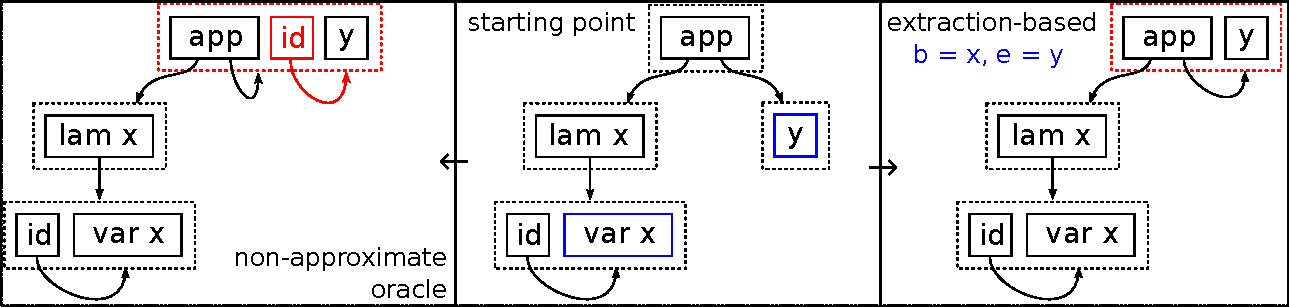
\includegraphics[width=0.9\linewidth]{media/extract-subs-example.pdf}
    \caption{Example of $\beta$-reduction with extraction-based substitution (right).
    The initial e-graph (middle) represents $(\lambda x.~id~x)~y$.
    After $\beta$-reduction, the e-graph does not represent $id~y$ because $x$ has been extracted for $b$ in the rewrite rule; ignoring $id~x$.}
    \label{fig:extract-subs}
\end{figure}

In practice, we have not observed the approximation to be an issue when optimizing \Rise{} programs (\cref{evaluation}), and believe that two main reasons account for this.
Firstly, the substitution is computed on each equality saturation iteration, where different terms may be extracted, increasing coverage of the set of terms represented by $b$ and $e$.
Secondly, many of the ignored equivalences are recovered either by e-graph congruence, or by applying further rewrite rules.
Future work may investigate alternative substitution implementations to balance efficiency with non-approximation.

\subsection{Name Bindings}
\label{name-bindings}

In equality saturation inappropriate handling of name bindings easily leads to serious efficiency issues.
Consider rewrite rules like \ref{map-fusion} that create a new lambda abstraction on their right-hand side.
What name should be introduced when they are applied?
In standard term rewriting, generating a fresh name using a global counter (aka. gensym) is a common solution.
But if a new name is generated each time the rewrite rule is applied, the e-graph is quickly burdened with many $\alpha$-equivalent terms\footnote{Two $\lambda$ terms are $\alpha$-equivalent if one can be made equivalent to the other simply by renaming variables.}.

Fewer $\alpha$-equivalent terms are introduced if fresh names are generated as a function of the matched e-class identifiers.
However as the e-graph grows and e-classes are merged, e-class identifiers change, and $\alpha$-equivalent terms are still generated and duplicated in the e-graph.

De Bruijn indices~\cite{DEBRUIJN1972381} are a standard technique for representing lambda calculus terms without naming the bound variables, and avoid the need for $\alpha$ conversions.
If De Bruijn indices enable two $\alpha$-equivalent terms to be structurally equivalent, the standard e-graph congruence invariant prevents their duplication, by ensuring that equivalent e-nodes are not allocated to different e-classes.
Hence we translate our terms and rewrite rules to use De Bruijn indices instead of names, and achieve significant efficiency gains (\cref{lambda-eval}).

\paragraph{True equality modulo $\alpha$-renaming}
While De Bruijn indices give a significant performance improvement, they do not provide equality modulo $\alpha$-renaming for sub-terms.
Consider  $f~(\lambda x.~f) = \%0~(\lambda.~\%1)$, where $\%i$ are De Bruijn indices.
Although $\%0$ and $\%1$ are structurally different, they both correspond to the same variable $f$.
In practice, we have not observed this to be a significant issue when optimizing \Rise{} programs, but it does require care when comparing sub-terms that have a different number of surrounding lambdas.
Future work may investigate alternatives to De Bruijn indices, for example through hashing modulo $\alpha$-renaming \cite{maziarz2021-hash-mod-alpha-eq}, or through nominal rewriting techniques \cite{fernandez2007-nominal-rewriting}.

\paragraph{Translating name-based rules into index-based rules}
Using De Bruijn indices means that rewrite rules must manipulate terms with De Bruijn indices.
Thankfully, more user-friendly name-based rewrite rules can be automatically translated to the index-based rules used internally \cite{bonelli2000-bruijn-rewriting}.
An example demonstrating this is given in \cref{rewrite-example}.

\paragraph{Explicit or extraction-based substitution}
Both explicit substitution and extraction-based substitution are compatible with De Bruijn indices, and for explicit substitution we use the $\lambda s$ calculus \cite{kamareddine1995-lambda-v}.

\paragraph{Shifting De Bruijn indices}
De Bruijn indices must be shifted when a term is used with different surrounding lambdas (example in \cref{rewrite-example}).
As for substitution, shifting can be implemented with explicit rewrite rules, or with \emph{extraction-based index shifting}:
\begin{itemize}
    \item extract a term from the e-class whose indices need shifting;
    \item perform index shifting on the term;
    \item add the resulting term to the e-graph.
\end{itemize}
In \kles{} we use extraction-based index shifting whenever extraction-based substitution is used.

\paragraph{Avoiding Name Bindings using Combinators}
It is also possible to avoid name bindings entirely \cite{smith2021-access-patterns}.
For example, it is possible to introduce a function composition combinator `$\circ$' as in \cref{eqsat}, greatly simplifying the \ref{map-fusion} and \ref{map-fission} rules:
\begin{align}
    \tag{$\circ$-intro}
    f~(g~x) &\rewritesTo{} (f \circ g)~x \\
    \tag{map-fusion$_2$}
    map~f \circ map~g &\rewritesTo{} map~(f \circ g) \\
    \tag{map-fission$_2$}
    map~(f \circ g) &\rewritesTo{} map~f \circ map~g
\end{align}

However, this approach has its own downsides.
Associativity rules are required, which we know increases the growth rate of the e-graph \cite{willsey2021-egg}.
Only using a left-/right-most associativity rule avoids generating too many equivalent ways to parenthesize terms.
But other rewrite rules now have to take this associativity convention into account, making their definition more difficult and their matching more expensive.
In general, matching modulo associativity or commutativity are algorithmically hard problems \cite{benanav1987-complexity-matching}.

The function composition $\circ$ combinator on its own is also not sufficient to remove the need for name bindings.
At one extreme, combinatory logic could be used as any lambda calculus term can be represented, replacing function abstraction by a limited set of combinators.
However, translating a lambda calculus term into combinatory logic results in a term of size $O(n^3)$ in the worst case, where $n$ is the size of the initial term \cite{lachowski2018-complexity}.
Translating existing rewrite systems to combinatory logic would be challenging in itself.
% Due to this potential term size explosion, and to the difficulty of translating an entire rewrite system to combinatory logic, we do not pursue this possibility further in this paper.

\subsection{Freshness Predicates}
\label{predicates}

Handling predicates is not trivial in equality saturation.
The \ref{eta-reduction} has the side condition that "$\text{if } x \text{ not free in } f$", but in an e-graph $f$ is an e-class and not a term.

The predicate could be precisely handled by filtering $f$ into $f' = \{ t \mid t \in f\text{, }x~\text{not free in}~t \}$, and using $f'$ on the right-hand-side of the rule.
However, this requires splitting an e-class in two: one that satisfies the predicate, and one that does not.
We do not attempt such a split as it would reduce sharing, increase e-graph size and be incompatible with the congruence invariant unless the very notion of equality is changed.

The design of \kles{} makes the engineering trade-off to only apply the \ref{eta-reduction} rewrite rule if $\forall t \in f.~x~\text{not free in}~t$, following egg's lambda calculus example \cite{willsey2021-egg}.
Advantages are that this predicate is efficient to compute using an e-class analysis, and that there is no need to split the e-class.
The disadvantage is that it is an approximation that ignores some valid terms.

\Cref{fig:missed-eta-example} shows an example where \ref{eta-reduction} is not applied.
In practice, we have not observed the approximation to be an issue, e.g.\ for the results presented in \cref{evaluation}.

\begin{figure}
    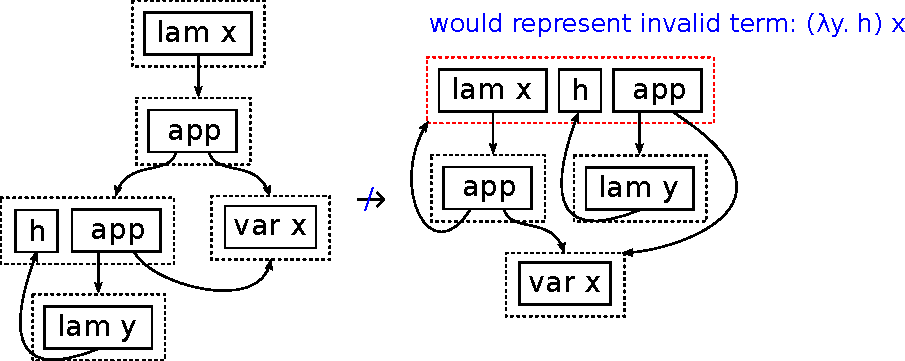
\includegraphics[width=0.55\linewidth]{media/eta-missed-example.pdf}
    \caption{Example where $\eta$-reduction is not applied.
    The initial e-graph represents $\lambda x.~h~x$, but $\eta$-reduction is not triggered because $h = (\lambda y.~h)~x$ where $x$ is free.
    Using $\exists$ instead of $\forall$ in our predicate, we would obtain the e-graph on the right which represents $h$, but also invalid terms such as $(\lambda y.~h)~x$ where $x$ is no longer bound.}
    \label{fig:missed-eta-example}
\end{figure}

\subsection{Adding Polymorphic Types}
\label{types}

Typed lambda calculi are pervasive, e.g.~as the foundation for almost all functional languages, and a key consideration is how to add types to the e-graph.
More specifically, we look at how polymorphic types interact with equivalence classes.
If types can be computed in a bottom-up fashion, an e-class analysis can be used, similar to how the size and shape of tensors is computed in \cite{wang2020-spores}.
However, if polymorphic types are monomorphized, their instantiation is context-dependent and cannot be computed in a bottom-up fashion.
For example, consider the terms $(\lambda x.~x)~(0: int)$ and $(\lambda x.~x)~(0.0: float)$.
In \Rise{}, the identify function is monomorphized and has two different type instantiations that should live in different e-classes: $\lambda x.~x : \text{int} \rightarrow \text{int}$ and $\lambda x.~x : \text{float} \rightarrow \text{float}$.
Hence, in \kles{} instantiated types are embedded in the e-graph instead of computed by an analysis.
Each e-class is associated with a type that all of its e-nodes must satisfy.

In an e-graph there is a tension between sharing and the availability of contextual information in a given e-class.
Type instantiation prevents sharing, as the same polymorphic expression produces a different e-class at each type. However, instantiation provides additional contextual information, as each e-class is associated with a precise monotype.

\paragraph{Hash-consing types}
Since types are duplicated many times in the e-graph, and since structural type equality is often required, we hash-cons types for efficiency \cite{filliatre2006-hashconsing}.
Alternatively, types could be stored in the e-graph itself to provide equational reasoning at the type level, but this is not necessary for this paper.

\subsection{Compiling user-defined rewrite rules}
\label{rewrite-example}

To avoid explicit typing or explicit use of De Bruijn indices in user-defined rewrite rules, user-friendly name-based and partially typed rewrite rules are compiled internally as required.

Types are inferred with \Rise{} type inference: both sides of rewrite rules can be seen as terms where free variables correspond to pattern variables.
After inferring the types on the left-hand-side, we check that the right-hand-side is well-typed for any well-typed left-hand-side match.
When applied, typed rewrite rules match (deconstruct) types with their left-hand-side, and construct types on their right-hand-side.
Type annotations can be used to constrain the inferred types.

Bound variables are replaced with their corresponding De Bruijn index, and indices are shifted as required for terms with differing numbers of surrounding lambdas.
We illustrate with examples.

\paragraph{Example 1:  $\eta$-reduction}

\begin{align*}
\lambda x.~f~x \quad\rewritesTo{}\quad& f &\text{if}~x~\text{not free in}~f
\end{align*}

\kles{} translates this rule into:
\begin{align*}
(\lambda. f~(\%0 :\ t_0)) :\ t_0 \to\ t_1 \quad\rewritesTo{}\quad& (\varphi^{-1}_1 f) :\ t_0 \to\ t_1 &\text{if}~\%0~\text{not free in}~f
\end{align*}
%(\lambda. ?0~(\%0 :\ ?t0)) :\ ?t0 \to\ ?t1 \rewritesTo{}& (\varphi^{-1}_1 ?0) :\ ?t0 \to\ ?t1 &\text{if}~x~\text{not free in}~f

The transformed rule uses a De Bruijn index $\%0$ for the bound variable, and pattern variables otherwise: $f$, $t_0$ and $t_1$. It provides index shifting through   $\varphi^{-1}_1 f$ that shifts all indices $\ge 1$ by $-1$ as a surrounding $\lambda$ has been removed.
Some types are matched on the left-hand-side ($t_0$ and $t_1$), and used to construct types on the right-hand-side ($t_0 \to t_1$).
Some types, like the type of $f$, are not matched on the left-hand-side as \kles{} avoids matching on redundant type information to some extent, assuming that the terms matched are well-typed.

\paragraph{Example 2: $\eta$-abstraction}

\begin{equation*}
f :\ t_0 \to t_1 \quad\rewritesTo{}\quad \lambda x.~f~x
\end{equation*}
$\eta$-abstraction illustrates how type annotations may be used, and are sometimes required.
\kles{} translates this rule into:
\begin{equation*}
f :\ t_0 \to t_1 \quad\rewritesTo{}\quad (\lambda.~(((\varphi^1_0 f) : t_0 \to t_1)~(\%0 : t_0)) :\ t_1) :\ t_0 \to t_1
\end{equation*}
A type error occurs if the type of $f$ is not annotated as in $f :\ t_0 \to t_1$ on the left-hand-side, since the right-hand-side requires it to be a function type. 